\documentclass[12pt]{article}

% Any percent sign marks a comment to the end of the line

% Every latex document starts with a documentclass declaration like this
% The option dvips allows for graphics, 12pt is the font size, and article
%   is the style

\usepackage[pdftex]{graphicx}
\usepackage{amsfonts}
\usepackage{amsmath}
\DeclareMathOperator*{\max_bottom}{max}
\usepackage{url}
\usepackage{hyperref}

\usepackage{caption}
\usepackage{subcaption}

\usepackage{graphicx}
\usepackage{amsmath}
\usepackage{adjustbox}
\usepackage{listings}

\lstset{language=python}

\hypersetup{
    colorlinks=true,
    linkcolor=blue,
    filecolor=magenta,      
    urlcolor=cyan,
    pdftitle={Sharelatex Example},
    bookmarks=true,
    pdfpagemode=FullScreen,
}


\usepackage{graphicx}
\graphicspath{ {./images/} }

% These are additional packages for "pdflatex", graphics, and to include
% hyperlinks inside a document.

\setlength{\oddsidemargin}{0.5cm}
\setlength{\evensidemargin}{0.5cm}
\setlength{\topmargin}{-1.6cm}
\setlength{\leftmargin}{0.5cm}
\setlength{\rightmargin}{0.5cm}
\setlength{\textheight}{24.00cm} 
\setlength{\textwidth}{15.00cm}
\parindent 0pt
\parskip 5pt
\pagestyle{plain}

% These force using more of the margins that is the default style
\newcommand{\namelistlabel}[1]{\mbox{#1}\hfil}
\newenvironment{namelist}[1]{%1
\begin{list}{}
    {
        \let\makelabel\namelistlabel
        \settowidth{\labelwidth}{#1}
        \setlength{\leftmargin}{1.1\labelwidth}
    }
  }{%1
\end{list}}


\begin{document}
\title{\Huge Introduction to machine learning - Homework 3}

\author{
  \textbf{Uri Kirstein}\\
  311137095 \\ sukirstn@campus.technion.ac.il
  \\ \\
  \textbf{Pavel Rastopchin}\\
  321082026 \\ pavelr@campus.technion.ac.il
  \\ \\ 
}

\maketitle


%\newpage
\section{Process and significant decisions}
\subsection{Using one model}
In Homework 3, during the automatic model selection, we found that the best model for the prediction tasks is a Multi-layer perceptron. In this homework we decided to use MLP model as well, according our findings. The main problem with sklearn MLP model was a high level of abstraction which prevented from us to use more advanced techniques. Thus, in this homework we will use Keras framework to build a deep learning model.   

\subsection{Minimal data pre-processing}
TODO

\subsection{Hyper parameters tuning with k-fold cross validation}
In order to select the best model, we need to perform k-fold cross validation using training set only. The cross validation process is implemented in cross Validator class. In all our cross-validation experiments we used the $accuracy$ and $f1_score$ as model performance measurement.

\subsection{Hyper parameters tuning with random search}
Based on Stanford CS231n course, lectures 6,7, we decided to use another technique for tuning the MLP parameters using random search, as this "brute force" technique might achieve better results than tuning parameters one by one.

\begin{figure}[h]
\centering
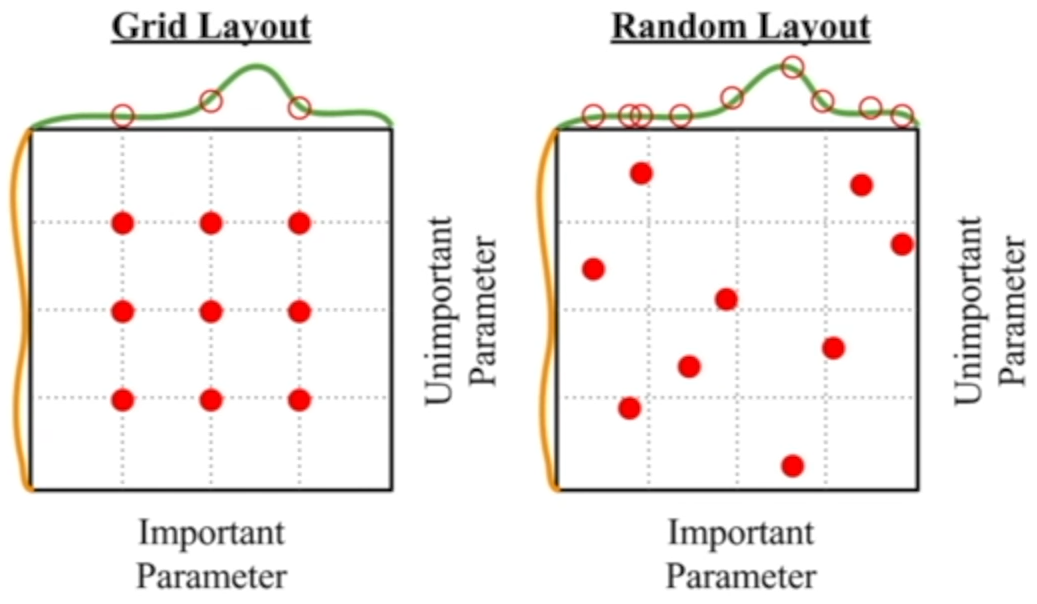
\includegraphics[width=.6\linewidth]{pics/random_search}
\caption{Random search of hyper-parameters}
\end{figure}


\section{MLP hyper-parameters tuning}
\subsection{Dropout probability}
\subsection{Leaky ReLU slope}
\subsection{Number of hidden layers}





\end{document}


\begin{figure}[h]
\centering
\begin{subfigure}{.5\textwidth}
  \centering
  \includegraphics[width=.6\linewidth]{Cross_valid_plots/SVM_C_hyper_fig_coarse.png}
  \caption{C coarse tuning}
  \label{fig:sub1}
\end{subfigure}%
\begin{subfigure}{.5\textwidth}
  \centering
  \includegraphics[width=.6\linewidth]{Cross_valid_plots/SVM_C_hyper_fig_fine.png}
  \caption{C fine tuning}
  \label{fig:sub2}
\end{subfigure}
\caption{Random search}
\label{fig:test}
\end{figure}

